\documentclass{article}
\usepackage[margin=0.80in, a4paper]{geometry} % Adjust margins here
\usepackage{amsmath}
\usepackage{float}
\usepackage{url} % For formatting URLs
\usepackage{hyperref}
\usepackage{subcaption}
\usepackage{graphicx} % subcaption for subfigure environment
%%%%%%%%%%%%%%%%%%%%%%%%%%%%%%%%%%%%%%%%%%%%%%%%%%%%%%%%%%%%%%%%%
\author{Francesco Angelo Fabiano Antonacci\\Francesco Sermi}

\date{\today}
\title{Relazione Natalizia}
%%%%%%%%%%%%%%%%%%%%%%%%%%%%%%%%%%%%%%%%%%%%%%%%%%%%%%%%%%%%%%%%%

\begin{document}
\maketitle

\section{Ricostruzione numerica di forme d'onda}
    \subsection{Forme d'onda quadre}
    \label{sez:quadra}
        Un'onda quadra alternata dispari con ampiezza picco-picco unitaria e fase 
        nulla è descitta dalla serie inifinita a Eq.($\ref{eq:quadra}$).

        \begin{equation}
            x(t) = \sum_{k=1,3,5...}^{\infty} \frac{2}{k\pi}\sin\left(k\omega t\right)
            \label{eq:quadra}
        \end{equation}


        \begin{figure}[htbp]
            \centering
            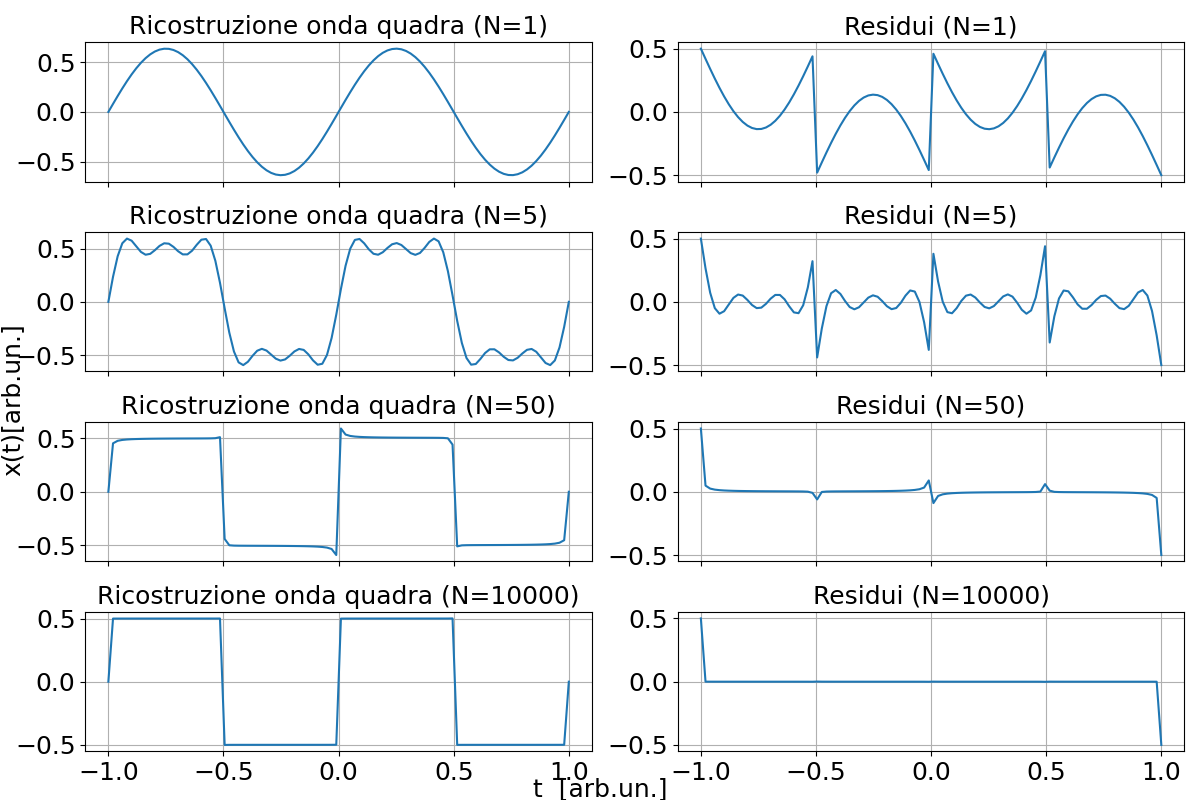
\includegraphics[width=1\textwidth]{fousquarewave1e2.png} % Replace with your image name
            \caption{A sinistra ricostruzione numerica dell'onda quadra Eq.($\ref{eq:quadra}$) su
                    due periodi con cento punti.
                    A destra residui tra onda analitica e la ricostruzione.
                    N è il numero a cui è stata troncata la serie.}
            \label{fig:quadra1e2}
        \end{figure}

        \noindent In Fig($\ref{fig:quadra1e2}$) e Fig($\ref{fig:quadra1e5}$) sono mostrate due ricostruzioni
        numeriche dell'onda quadra.
        All'aumentare dei termini $N$ della serie diminuisce la distranza tra onda analitica e serie 
        di seni.

        \noindent Si osserva che nel caso di Fig($\ref{fig:quadra1e2}$),
        la quale ha una risoluzion  peggiore, la deformazione dell'onda quadra assomiglia a quanto visto nelle esperienze 
        pratiche di laboratorio con l'oscilloscopio quando si usa il generatore di funzioni a
        frequenze sufficientemente alte: forse questo rivela qualcosa sul funzionamento del generatore
        di funzioni.\\

        \begin{figure}[htbp]
            \centering
            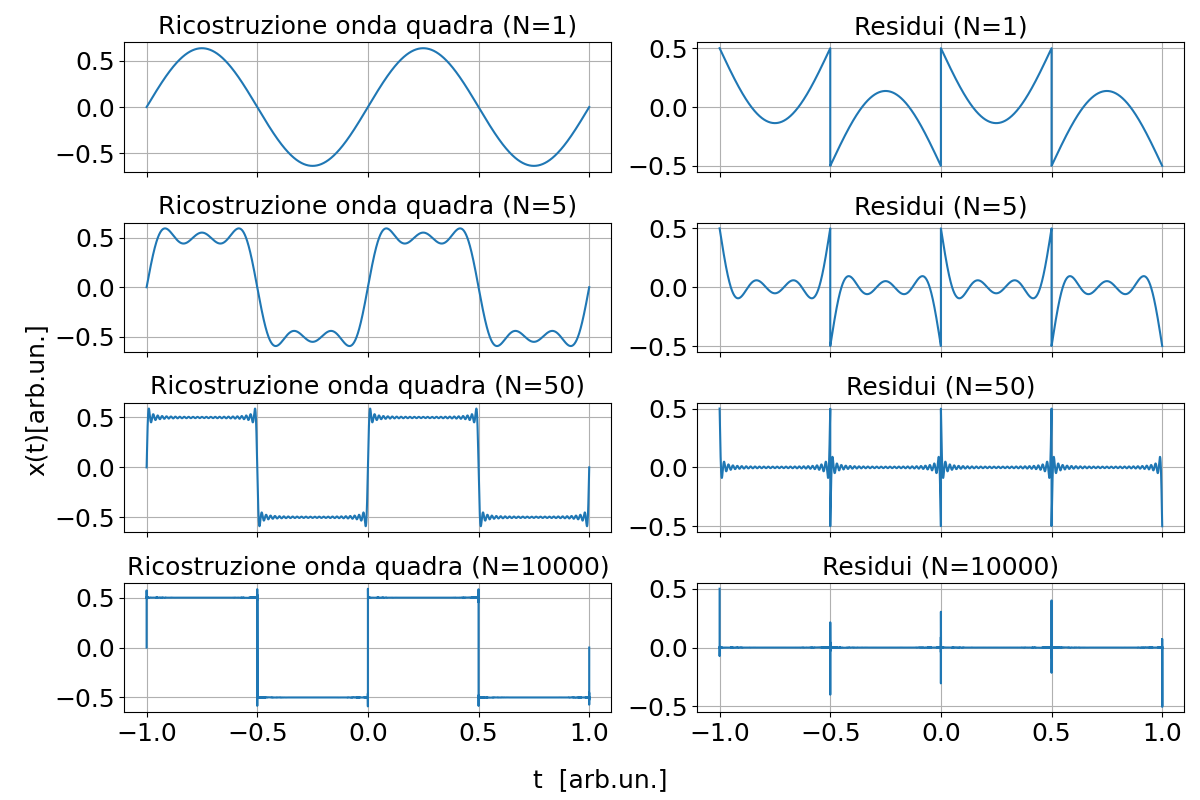
\includegraphics[width=1\textwidth]{fousquarewave1e5.png} % Replace with your image name
            \caption{A sinistra ricostruzione numerica dell'onda quadra Eq.($\ref{eq:quadra}$) su
                    due periodi con centomila punti.
                    A destra residui tra onda analitica e la ricostruzione.
                    N è il numero a cui è stata troncata la serie.}            \label{fig:quadra1e5}
        \end{figure}  
        
        
        \noindent Si osserva che la presenza di lati obliqui nei transienti è conseguenza di un sottocampionamento
        della mia ricostruzione, questo comporta che non c'è miglioramento all'aumentare dei termini 
        della serie.

        \noindent I residui nei punti iniziali e i transienti non si annullano mai: in corrispondenza di ognuno di
        questi punti si trovano dei picchi. \newline \newline


    \subsection{Forme d'onda triangolari}
        Un'onda triangolare alternata pari con ampiezza picco-picco unitaria
        e fase nulla è descitta dall' Eq.($\ref{eq:triangolare}$).
        \begin{equation}
            x(t) = \sum_{k=1,3,5...}^{\infty} \left(\frac{2}{k\pi}\right)^{2}\cos\left(k\omega t\right)
            \label{eq:triangolare}
        \end{equation}


        \begin{figure}[H]
            \centering
            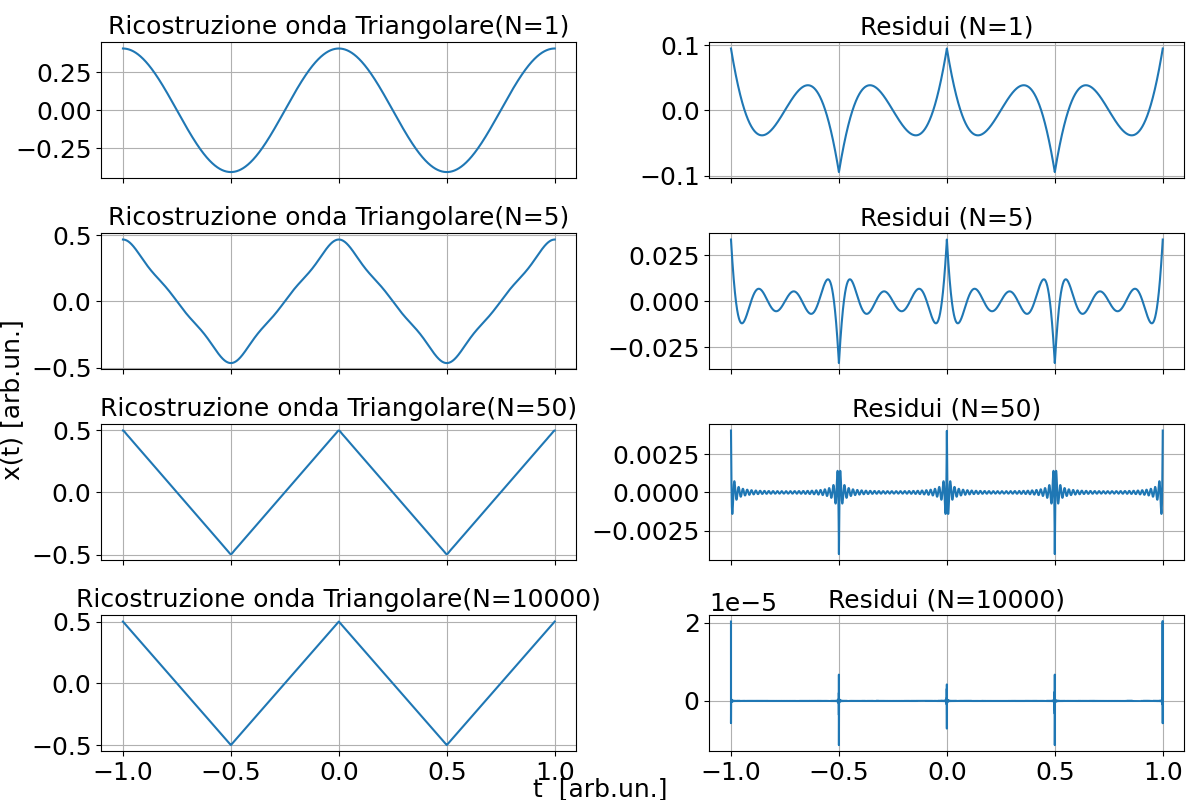
\includegraphics[width=1\textwidth]{foutriawave1e5.png} % Replace with your image name
            \caption{A sinistra ricostruzione numerica dell'onda triangolare
             Eq.($\ref{eq:triangolare}$) su due periodi con centomila punti.
            A destra residui tra onda analitica e la ricostruzione.
            N è il numero a cui è stata troncata la serie. }
            \label{fig:trian1e5}
        \end{figure}
        \noindent Similmente a quanto accade per l'onda quadra, anche in questo caso, nei punti 
        in cui la derivata è discontinua e nei punti al bordo non c'è convergenza
        semplice come si può vedere dai grafici dei residui in Fig.($\ref{fig:trian1e5}$) e 
        Fig.($\ref{fig:trian1e2}$).
        Anche solo qualitativamente si osserva a entrambe le risolizioni che 
        la convergenza all'onda analitica è più rapida dell'onda quadra, una migliore discussione di ciò avverrà in
        Sez.($\ref{sez:residui}$).
        \begin{figure}[H]
            \centering
            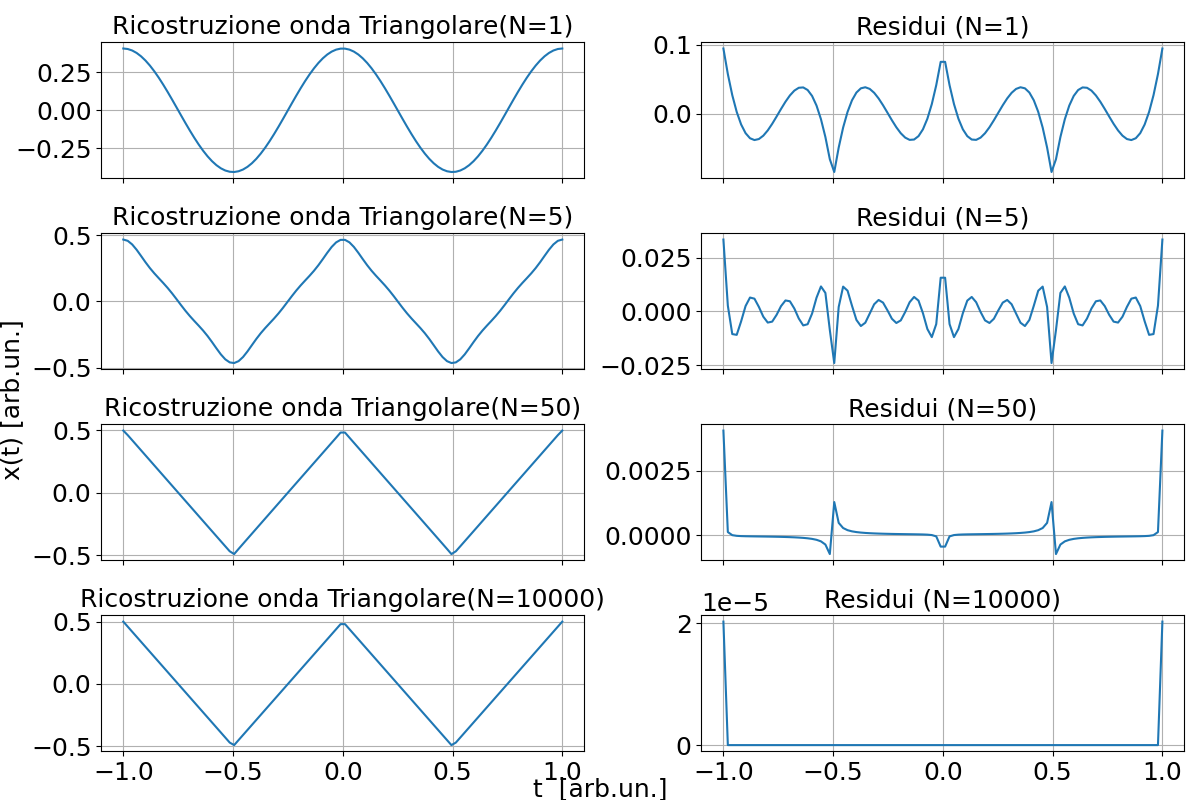
\includegraphics[width=1\textwidth]{foutriawave1e2.png} % Replace with your image name
            \caption{A sinistra ricostruzione numerica dell'onda triangolare
            Eq.($\ref{eq:triangolare}$)su due periodi con cento punti.
           A destra residui tra onda analitica e la ricostruzione.
           N è il numero a cui è stata troncata la serie. }
            \label{fig:trian1e2}
        \end{figure}        
        
        \noindent Per quanto riguarda l'utilizzo di diverse risoluzioni nei grafici, l'impiego di una risoluzione 
        minore comporta problemi nella convergenza solo nei punti iniziali e non nei punti di transiente,
        l'impiego di una risoluzione maggiore fa osservare dei picchi nei residui in prossimità dei transienti.
        Chiaramente non mettere i punti di picco tra i punti che vengono campionati 
        comporta una deformazione della forma d'onda graficata che non viene osservata 
        nei residui.




    \subsection{Verifica di convergenza della serie}
    \label{sez:residui}
       
        La serie di Fourier delle rispettive onde dovrebbe convergere integralmente alle funzioni analitiche.
        Come ci si aspetta dalla teroria, la velocità di convergenza rispetto al numero 
        di iterazioni è diversa per le forme d'onda come si può vedere 
        in Fig.($\ref{fig:res1}$).\\ 
        Tuttavia nel caso dell'onda quadra si osserva un comportamento inaspettato:
        quando il campionamento avviene su numero sufficientemente
        piccolo di periodi,  non c'è più convergenza integrale tra la funzione semplice, definita sugli 
        intervalli dalla serie di Fourier, e la funzione analitica:con ogni
        probabilità questo è dovuto al transiente che non è adeguatamente approssimato.
        Inoltre,per entrambe le onde compiono delle oscillazioni dei residui che si
        smorzano nella coda all'aumentare delle iterazioni come 
        si può vedere in Fig.($\ref{fig:res2}$).
        

        \begin{figure}[H]
            \centering
            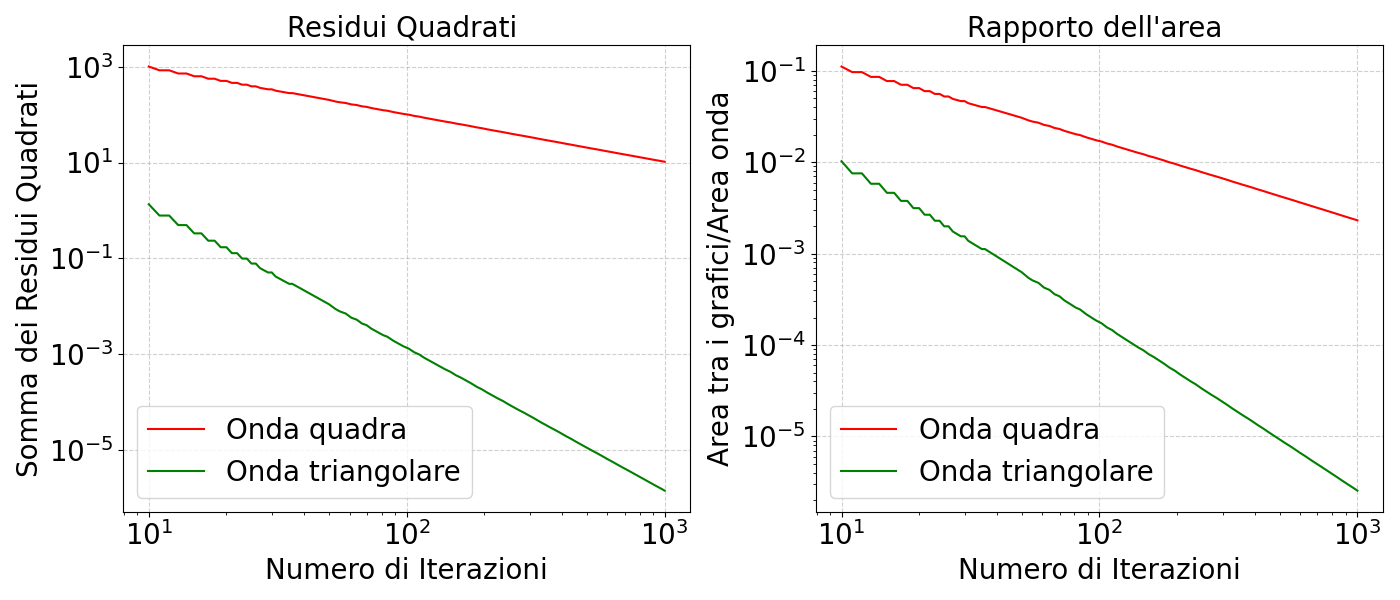
\includegraphics[width=1\textwidth]{residuals1.png} % Replace with your image name
            \caption{Nella figura simulazione numerica sono stati usati cento milioni di campionamenti presi tra due periodi.}
            \label{fig:res1}
        \end{figure}

      

        \begin{figure}[H]
            \centering
            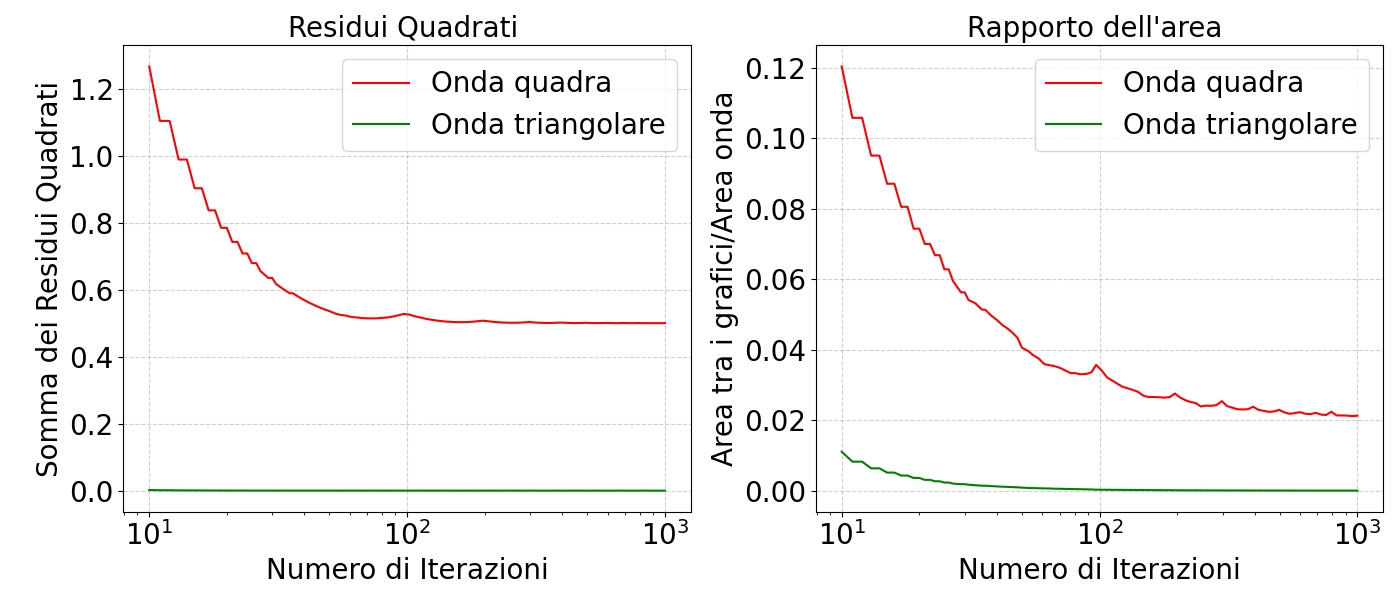
\includegraphics[width=1\textwidth]{residuals2.png} % Replace with your image name
            \caption{Nella figura simulazione numerica sono stati usati 100 campionamenti presi tra due periodi.}
            \label{fig:res2}
        \end{figure}

    \subsection{Treni di impulsi}
    Un treno di impulsi pari con ampiezza picco-picco unitaria e fase nulla è descitta
    dall' Eq.($\ref{eq:ciufciuf}$).

    \begin{equation}
        x(t) = \sum_{k=1,3,5...}^{\infty} \left(\frac{2}{k\pi}\right)\sin\left(k\pi\delta\right)\cos\left(k\omega t\right)
        \label{eq:ciufciuf}
    \end{equation}
    $\delta$ è il rapporto tra massimo e minimo dell'onda.
    Come si può vedere in Fig.($\ref{fig:ciufciuf1} $) e in Fig.($\ref{fig:ciufciuf2} $)
    si possono fare le stesse identiche osservazioni fatte in Sez(\ref{sez:quadra}).
    \begin{figure}[H]
        \centering
        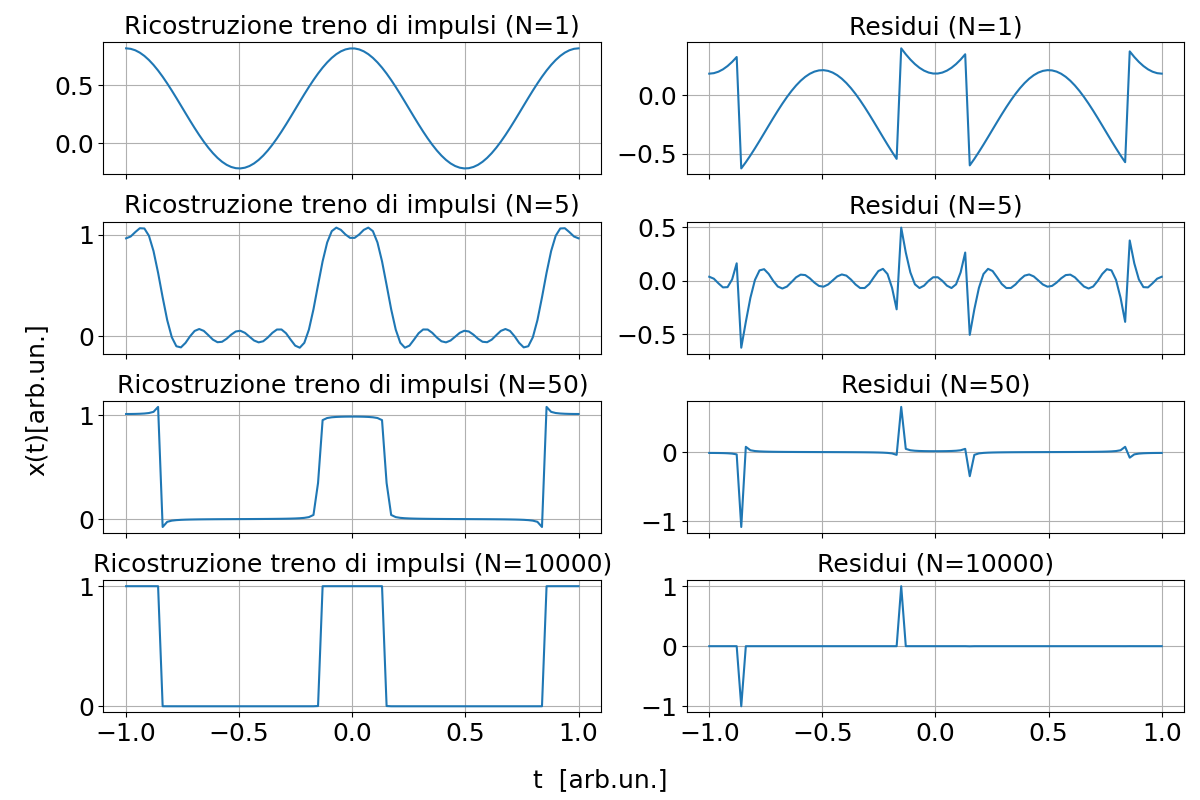
\includegraphics[width=1\textwidth]{foupulsetrainwave1e2.png} % Replace with your image name
        \caption{A sinistra ricostruzione numerica del treno di impulsi
        Eq.($\ref{eq:ciufciuf}$)su due periodi con cento punti.
        A destra residui tra onda analitica e la ricostruzione.
        N è il numero a cui è stata troncata la serie. }
        \label{fig:ciufciuf1}
    \end{figure}

    \begin{figure}[H]
        \centering
        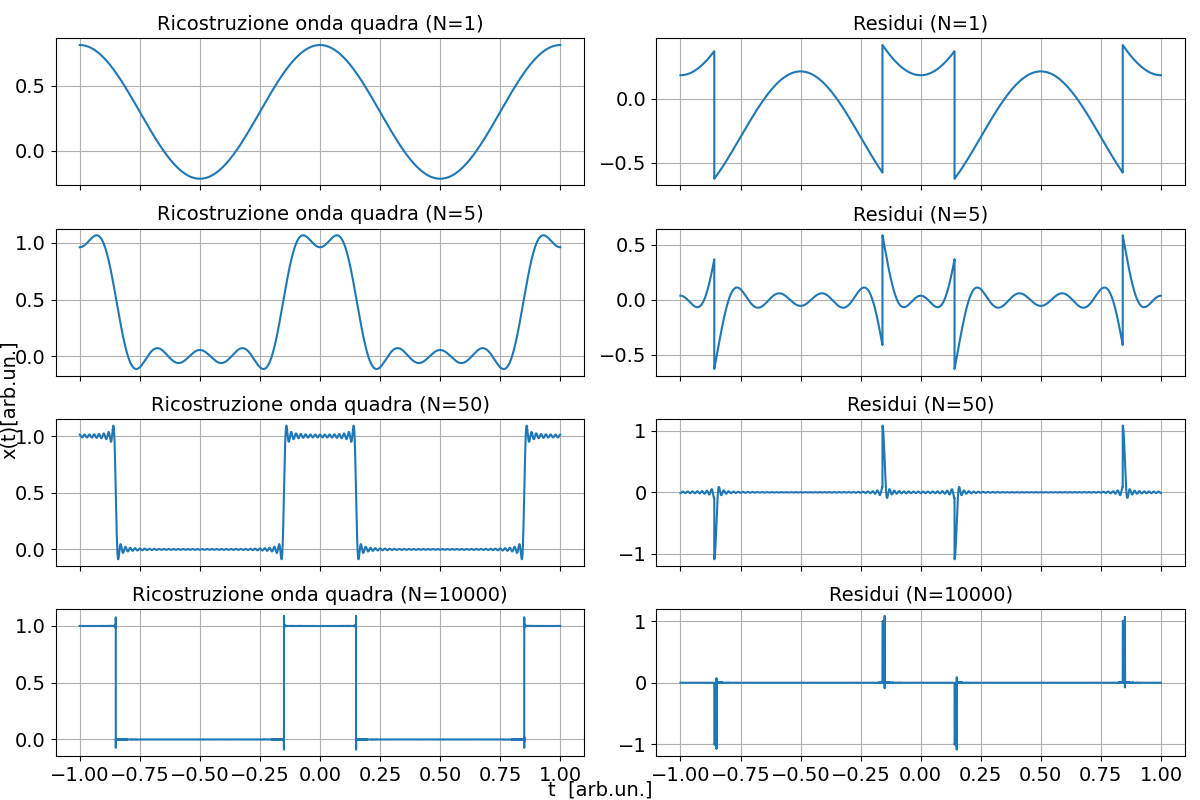
\includegraphics[width=1\textwidth]{foupulsetrainwave1e5.png} % Replace with your image name
        \caption{A sinistra ricostruzione numerica del treno di impulsi
        Eq.($\ref{eq:ciufciuf}$)su due periodi con centomila punti.
        A destra residui tra onda analitica e la ricostruzione.
        N è il numero a cui è stata troncata la serie. }
        \label{fig:ciufciuf2}
    \end{figure}



\section{Filtro passa basso e filtro passa alto}
    \label{sez:filt}
    Un filtro passa basso di frequenza di taglio $f_T$, che riceve un segnale sinusoidale, di 
    frequenza angolare $\omega$,lo riscala di un fattore $G$ e lo sfasa di un 
    angolo $\phi$ come dato da Eq.($\ref{eq:lpf}$).
        \begin{equation}
            f = \frac{\omega}{2\pi}, \quad 
            G(f) = \frac{1}{\sqrt{1 + \left(\frac{f}{f_T}\right)^2}}, \quad 
            \phi = \arctan\left(\frac{-f}{f_T}\right)
            \label{eq:lpf}
        \end{equation}
    Un filtro passa alto di frequenza di taglio $f_T$, che riceve un segnale sinusoidale, di 
    frequenza angolare $\omega$,lo riscala di un fattore $G$ e lo sfasa di un 
    angolo $\phi$ come dato da Eq.($\ref{eq:hpf}$).
        \begin{equation}
            f = \frac{\omega}{2\pi}, \quad 
            G(f) = \frac{1}{\sqrt{1 + \left(\frac{f_T}{f}\right)^2}}, \quad 
            \phi(f)= \arctan\left(\frac{f_T}{f}\right)
            \label{eq:hpf}
        \end{equation}

    Dunque le equazioni per le onde passanti per ciascuno dei filtri si trovano
    moltiplicando ciascun termine della sommatoria per il rispettivo 
    $G \left( k\omega,f_T\right)$ e sommando il termine $\phi \left( k\omega,f_T\right)$ 
    all'interno della sinusoide o cosinusoide. $G$ e $\phi$ hanno significato di Eq.($\ref{eq:lpf}$)
    o Eq($\ref{eq:hpf}$) dipendentemente dal filtro del contesto.
      

    
    \subsection{Onda quadra}
    Le funzioni descriventi il segnale i uscita o in ingresso da un filtro passa basso
    o passa alto, i quali in ingresso hanno un'onda quadra, 
    sono date dal procedimento descritto i Sez.($\ref{sez:filt}$).
        \subsubsection{Filtro passa basso}
            \label{sez:int_quadra}
            Come nella sezione precedente, è possibile verificare la convergenza della serie di 
            seni con la forma d'onda analitica.
            Inoltre, si possono fare le stesse considerazioni riguardanti 
            il numero di termini della serie impiegati, i transienti e il campionamento
            (vedi Fig($\ref{fig:shark1e2}$) e Fig($\ref{fig:shark1e5}$)).
                    \begin{figure}[H]
                        \centering
                        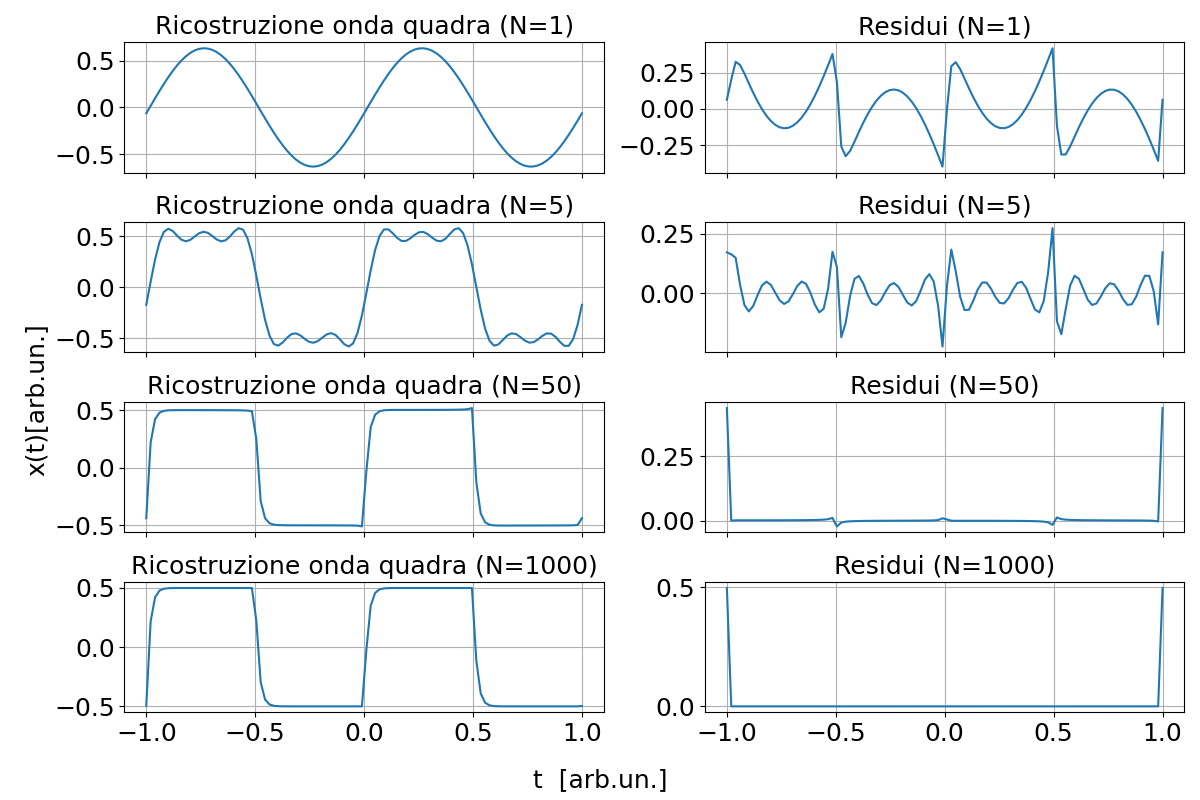
\includegraphics[width=1\textwidth]{fousharkfins1e2.png} % Replace with your image name
                        \caption{A destra c'è l'onda a pinna di squalo.
                        A sinistra c'è il grafico dei residui.
                        La risoluzione utilizzata è stata di cento punti su due periodi.}
                        \label{fig:shark1e2}
                    \end{figure}
                    \begin{figure}[H]
                        \centering
                        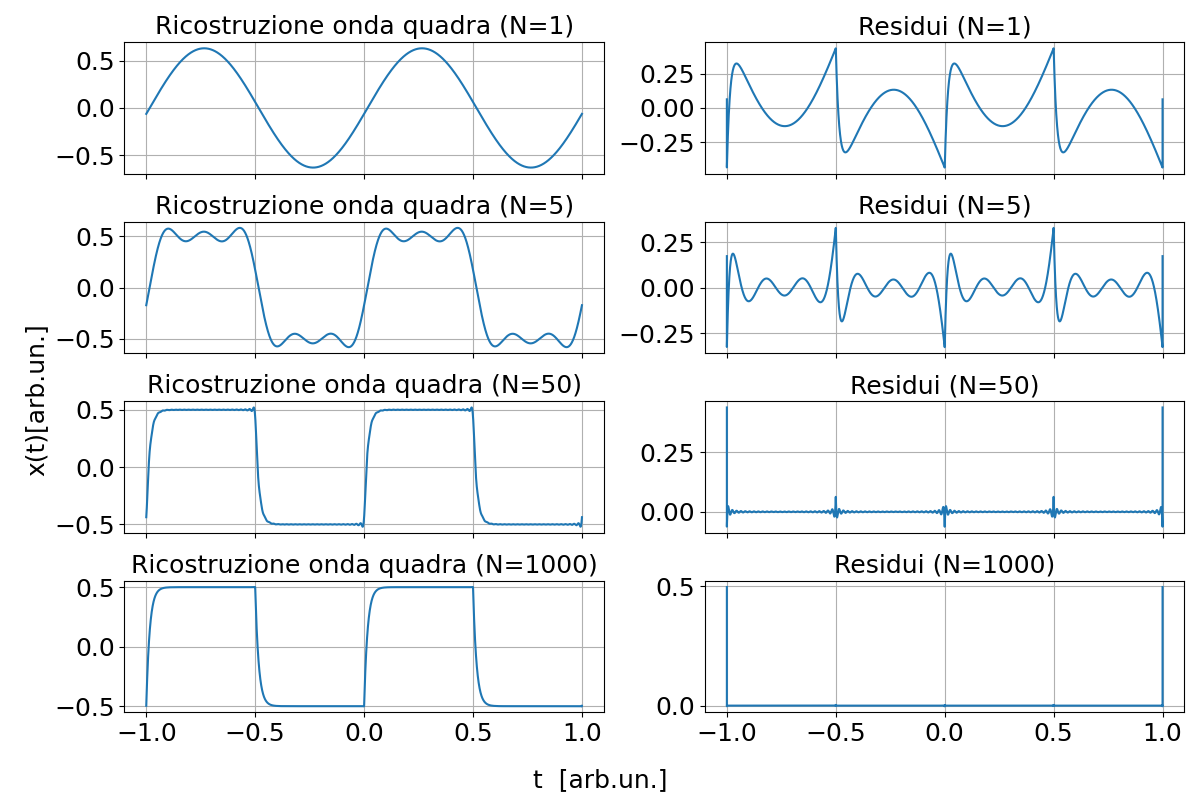
\includegraphics[width=1\textwidth]{fousharkfins1e5.png} % Replace with your image name
                        \caption{A destra c'è l'onda a pinna di squalo.
                        A sinistra c'è il grafico dei residui.
                        La risoluzione utilizzata è stata di centomila punti su due periodi.
                        La serie di Fourier è stata troncata al termine $N=10000$.}
                        \label{fig:shark1e5}
                    \end{figure}
                Si può facilmente simulare il comportamento di  un filtro al
                variare della frequenza in ingresso: per semplicità 
                la simulazione è stata fatta tenendo fissa la frequenza dell'onda e 
                variando la frequenza di taglio, come fatto in Fig.($\ref{fig:sharkft}$).
                    \begin{figure}[H]
                        \centering
                        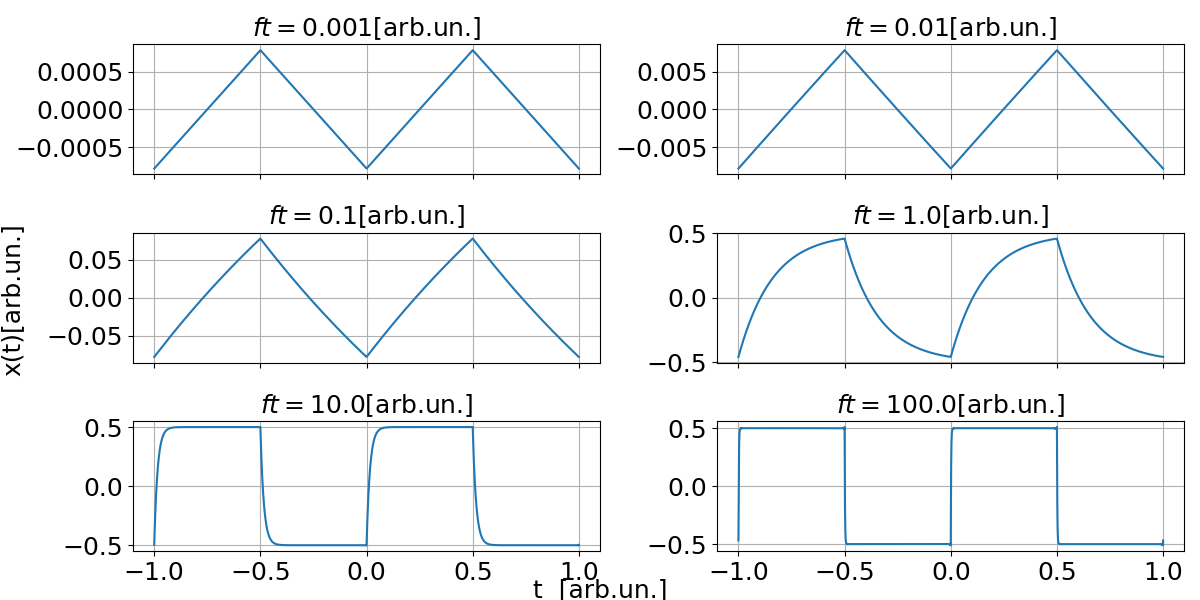
\includegraphics[width=1\textwidth]{fousharkfinsfts1.png} % Replace with your image name
                        \caption{Onde a pinna di squalo al variare della frequenza di taglio.
                        La risoluzione utilizzata è stata di centomila punti su due periodi.
                        La serie di Fourier è stata troncata al termine $N=10000$.}
                        \label{fig:sharkft}
                    \end{figure}

                \noindent Si vede chiaramente che quanto simulato è in accordo con quanto
                visto in laboratorio: 
                al decrescere della frequenza di taglio rispetto alla frequenza dell'onda quadra
                l'onda tende a diventare triangolare e la sua ampiezza diminuisce; viceversa,
                l'onda tenda a divenire quadra, ossia il segnale in ingresso tende a 
                rimanere inalterato.
            
            
            \subsubsection{Filtro passa alto}
                E'interessante simulare il comportamento di un filtro passa alto 
                come fatto in Fig($\ref{fig:der_square}$): si  può osservare specialmente 
                nel caso $ft=0.1$[arb.un.] la stessa forma d'onda osservata collegando 
                l'oscilloscopio in modalità AC al generatore di funzioni.
                    \begin{figure}[H]
                        \centering
                        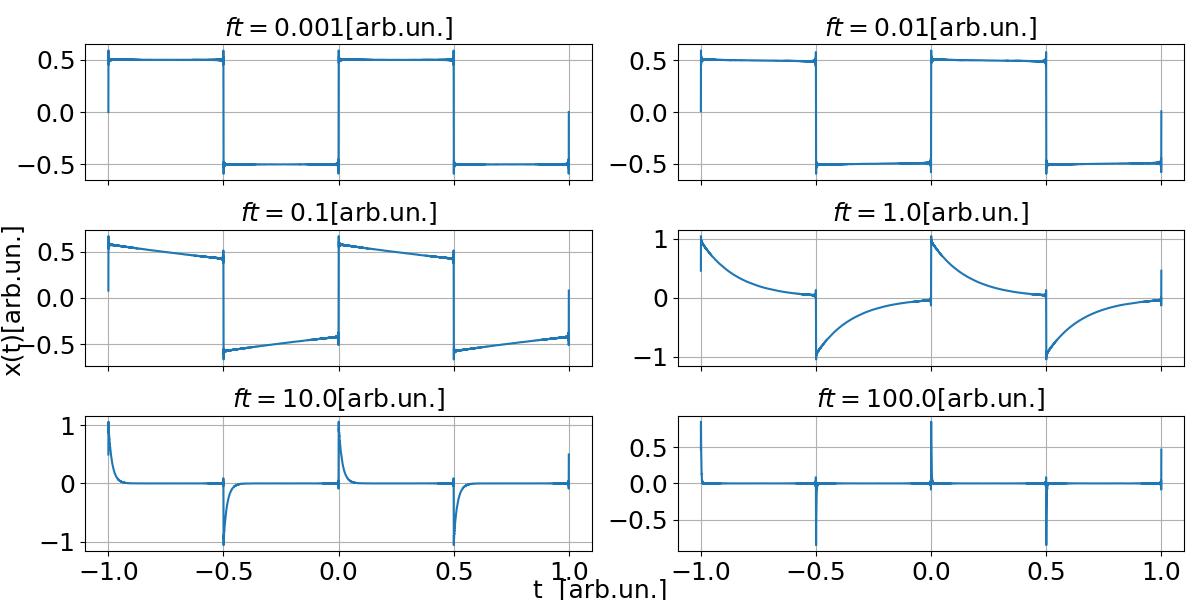
\includegraphics[width=1\textwidth]{der_square.png} % Replace with your image name
                        \caption{Simulazione di filtro passa alto con onda quadra.
                        La risoluzione utilizzata è stata di centomila punti su due periodi.
                        La serie di Fourier è stata troncata al termine $N=10000$.}
                        \label{fig:der_square}
                    \end{figure}


    \subsection{Onda triangolare}
    Le funzioni descriventi il segnale i uscita o in ingresso da un filtro passa basso
    o passa alto, i quali in ingresso hanno un'onda triangolare, 
    sono date dal procedimento descritto i Sez.($\ref{sez:filt}$).
        \subsubsection{Integratore}
            
            In Fig.($\ref{fig:trilpf}$) anche il comportamento di un filtro passa
            basso per un onda triangolare. Valgono tutti i commenti precedentemente in 
            Sez.($\ref{sez:int_quadra}$)
            \begin{figure}[H]
                \centering
                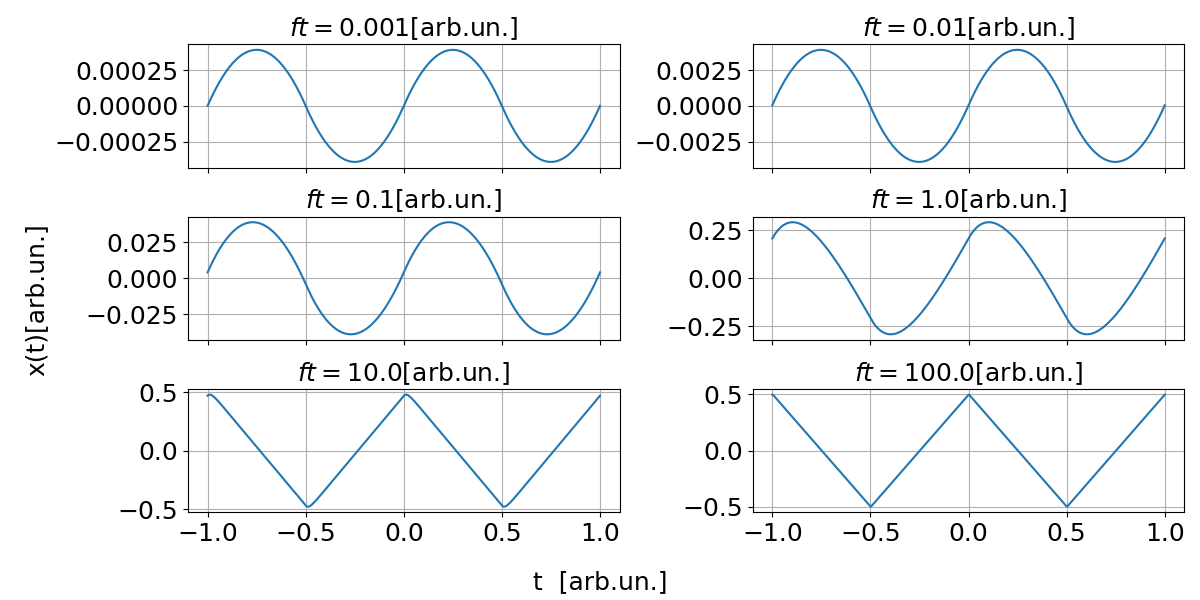
\includegraphics[width=1\textwidth]{integ_trian.png} % Replace with your image name
                \caption{Per la ricostruzione della forma d'onda è stato adottato 
                il procedimento descritto in Sez.($\ref{sez:filt}$).
                La risoluzione utilizzata è stata di centomila punti su due periodi.
                La serie di Fourier è stata troncata al termine $N=10000$.}
                \label{fig:trilpf}
            \end{figure}
        \subsubsection{Derivatore}
            In questo caso si osserva (vedi Fig.($\ref{fig:trihpf}$))che la forma d'onda 
            triangolare passante per un filtro passa alto coincide con quella simulata 
            per un filtro passa basso attraversato da un'onda quadra(vedi Fig($\ref{fig:sharkft}$))
                \begin{figure}[H]
                    \centering
                    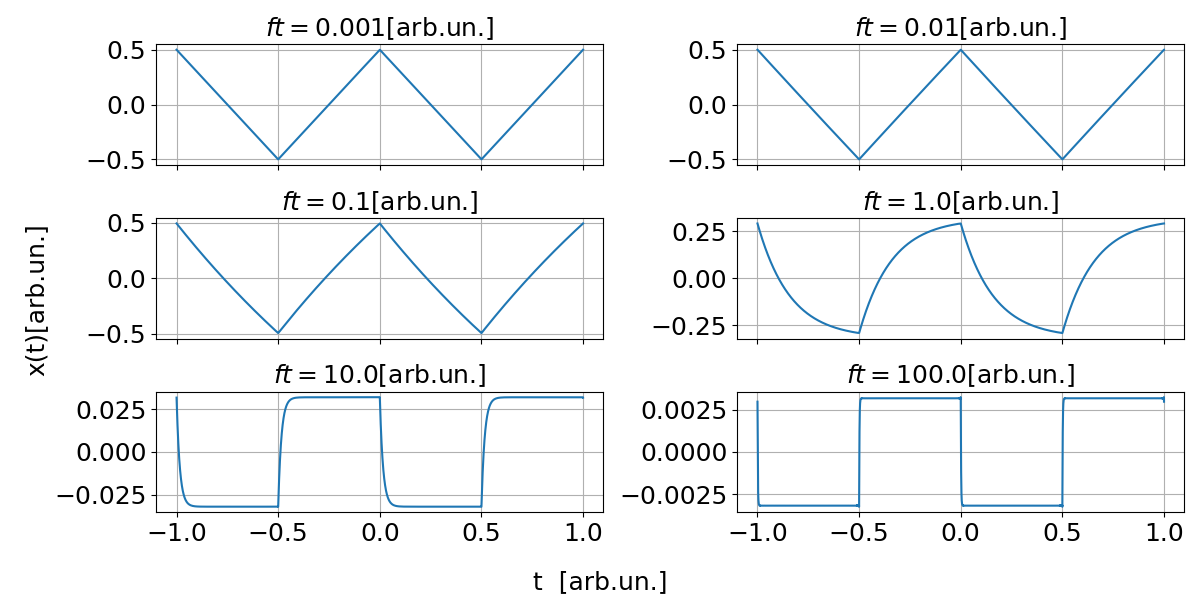
\includegraphics[width=1\textwidth]{der_trian.png} % Replace with your image name
                    \caption{Per la ricostruzione della forma d'onda è stato adottato 
                    il procedimento descritto in Sez.($\ref{sez:filt}$).
                    La risoluzione utilizzata è stata di centomila punti su due periodi.
                    La serie di Fourier è stata troncata al termine $N=10000$.}
                    \label{fig:trihpf}
                \end{figure}


    \subsection{Treno di impulsi}
    Le funzioni descriventi il segnale i uscita o in ingresso da un filtro passa basso
    o passa alto, i quali in ingresso hanno un treno di impulsi, 
    sono date dal procedimento descritto i Sez.($\ref{sez:filt}$).
  
            \subsubsection{Integratore}
            Le osservazioni che si possono fare in questo caso sono già state fatte 
            nella trattazione dell'onda quadra Sez.($\ref{sez:int_quadra}$).
            In Fig.($\ref{fig:int_train}$) viene riportato il segnale integrato di un treno di impulsi.
                Per facilità di rappresentazione e facilitare possibili manipolazioni
                nello studio della forma, è stato scelto di tenere compresa la forma 
                d'onda in un intervallo unitario centrato in zero.
                Se questo non fosse stato fatto appositamente, la forma d'onda, non 
                essendo alternata, non avrebbe spontaneamente, eccetto che nel caso 
                in cui si fosse ricondotti a un'onda quadra, rispettato questa richiesta.
        
                    \begin{figure}[H]
                        \centering
                        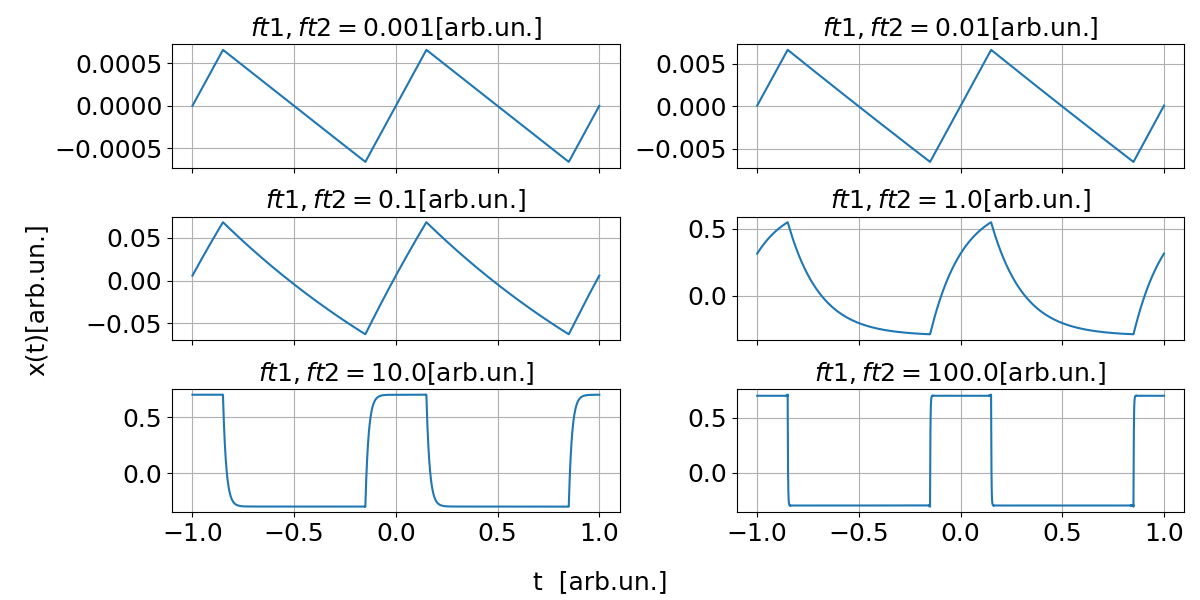
\includegraphics[width=1\textwidth]{int_train1.png} % Replace with your image name
                        \caption{Per la ricostruzione della forma d'onda è stato adottato 
                        il procedimento descritto in Sez.($\ref{sez:filt}$).
                        La risoluzione utilizzata è stata di centomila punti su due periodi.
                        E' stato fatto un troncamento al tremine 10000
                        nello sviluppo della serie di seni.}
                        \label{fig:int_train}
                    \end{figure}               

            \subsubsection{Derivatore}
                In Fig.($\ref{fig:der_train}$) viene riportato il segnale derivato di un treno di impulsi.     
                    
                    \begin{figure}[H]
                        \centering
                        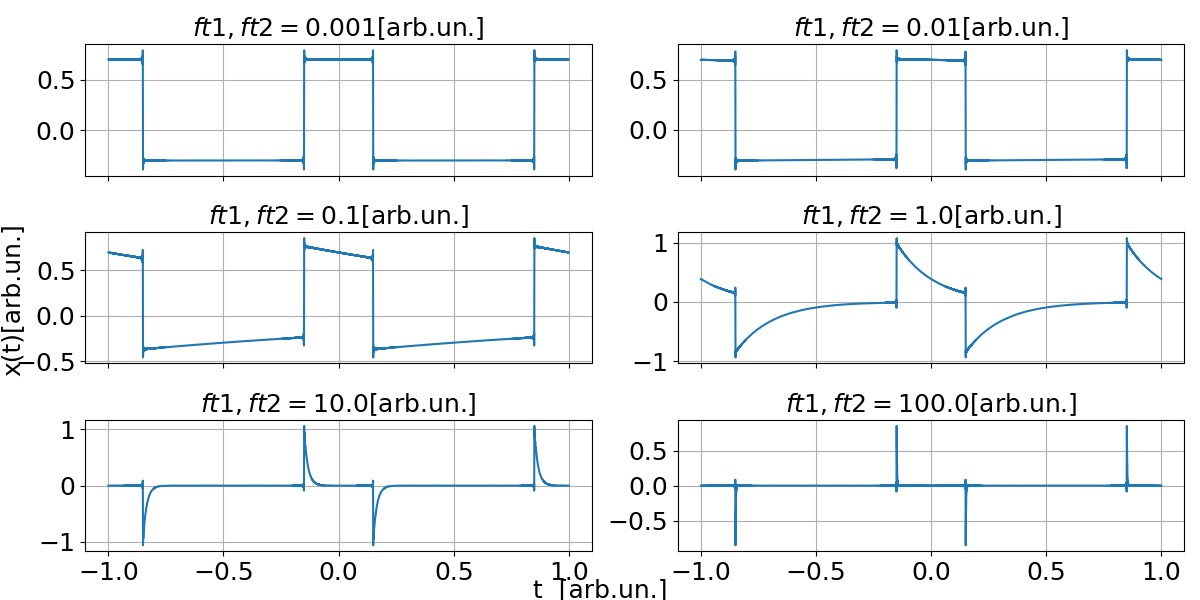
\includegraphics[width=1\textwidth]{der_train.png} % Replace with your image name
                        \caption{Per la ricostruzione della forma d'onda è stato adottato 
                        il procedimento descritto in Sez.($\ref{sez:filt}$).
                        La risoluzione utilizzata è stata di centomila punti su due periodi.
                        Sono stati usati 10000 termini della serie di seni.}
                        \label{fig:der_train}
                    \end{figure}    

            \subsubsection{Filtro passa banda}
                E' adesso pura questione di soddisfazione simulare l'effetto
                di un filtro passabanda su un terno di impulsi. Si veda Fig.($\ref{fig:band_train}$).
                \begin{figure}[H]
                    \centering
                    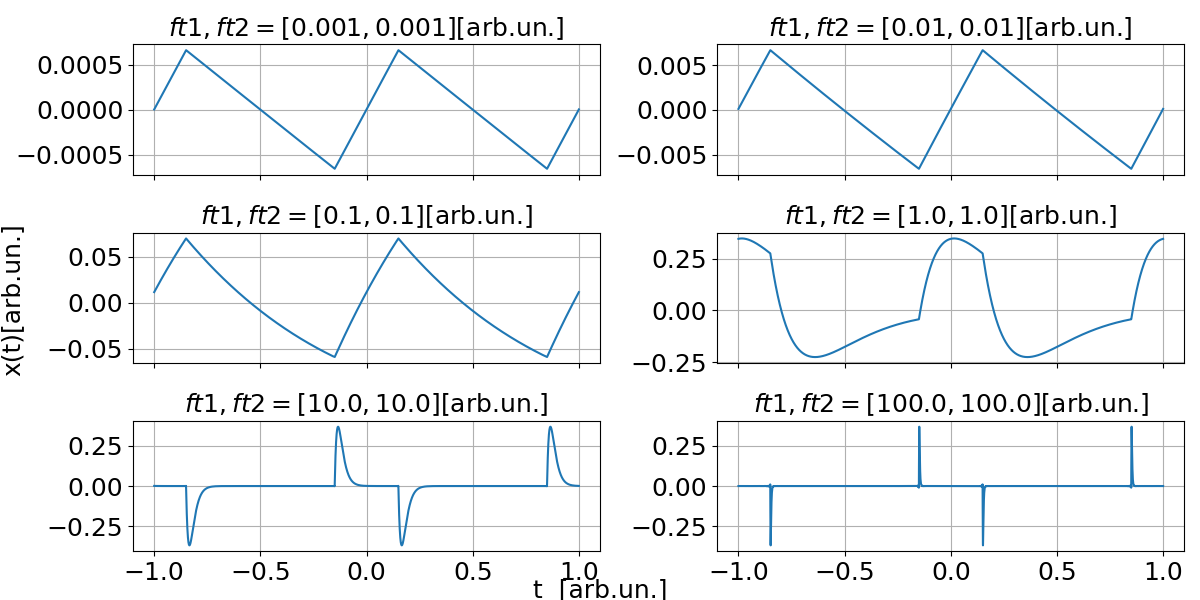
\includegraphics[width=1\textwidth]{band_train.png} % Replace with your image name
                    \caption{Per la ricostruzione della forma d'onda è stato adottato 
                    il procedimento descritto in Sez.($\ref{sez:filt}$).
                    La risoluzione utilizzata è stata di centomila punti su due periodi.
                    Sono stati usati 10000 termini della serie di seni.}
                    \label{fig:band_train}
                \end{figure}


\section{Best fit dei dati acquisiti con Arduino}
    Per tutti i best-fit realizzati è stato utilizzato mille come numero con cui 
    troncare la serie di Fourier. Questo è stato necessario per far eseguire il 
    best-fit in tempi ragionevoli.
    Come incertezza sulle misure di potenziale è stata
    presa la deviazione standard campione di un set di dati di misure
    di differenze di potenziale costante raccolti con Arduino \cite{Antonacci_Sermi2024}.
    
    \subsection{Onda quadra}
            E' stato realizzato il best-fit dei minimi quadrati
            di un set di dati compatibile con un'onda quadra.
            Il modello con cui fare il best-fit è descritto dall'Eq.($\ref{eq:fit_square}$).
                \begin{equation}
                    V(t) = \left[a\sum_{k=1,3,5...}^{1000} \frac{2}{k\pi}\sin\left(k\omega (t+\delta)\right)\right] +c
                    \label{eq:fit_square}
                \end{equation}
            Si osserva che trascurare o meno i punti sui transienti è incisivo
            sul risultato di best-fit come si può vedere in Fig.($\ref{fig:bestfit_square}$ ).
            E' stato dunque ragionevole utilizzare $absolute\_ sigma=True$
            nel primo best fit, e $absolute\_ sigma=False$ nel secondo.
            Dal $\chi^2$ risulta che l'errore è stato sovrastimato. 
            I parametri ottenuti sono riportati in Tab.(\ref{tab:bestfit_square}).
            In Fig.($\ref{fig:bestfit_square}$) sono riportati i dati con il best fit e 
            i residui.
            

            \begin{figure}[H]
                \centering
                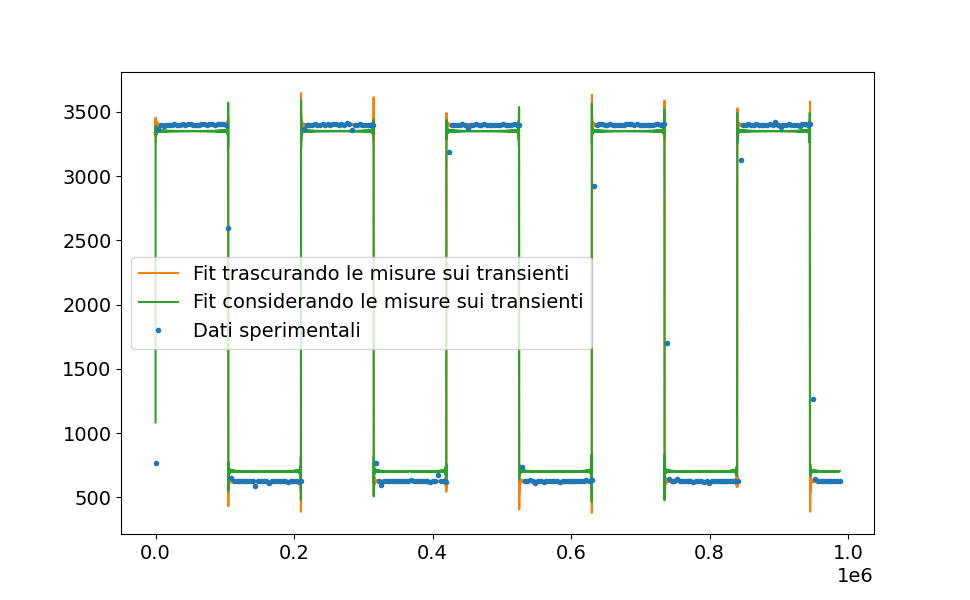
\includegraphics[width=1\textwidth]{bestfit_squarewave.png} % Replace with your image name
                \caption{                }
                \label{fig:bestfit_square}
            \end{figure}     
            

            \begin{table}[H]
                \centering
                \begin{tabular}{ccc}
                    \hline
                     & Fit trascurando i transienti & Fit considerando i transienti \\
                    \hline
                    $\omega$ [rad/s]        & $29.923 \pm 0.001$    & $29.930\pm 0.003$ \\
                    $\delta$ [$\mu$s]       & $-35\pm 24$           & $-42\pm 19$ \\
                    a [arb.un]              & $2774 \pm 1$          & $2647 \pm 47$ \\
                    c [arb.un]              & $2012.8 \pm 0.7$      & $2026 \pm 23$ \\
                    $\chi^{2}_{norm}$ & 0.01 & 14 \\
                    \hline
                \end{tabular}
                \caption{Parametri ottenuti nei best-fit dell'onda quadra. 
                Vedi modello Eq.($\ref{eq:fit_square}$).}
                \label{tab:bestfit_square}
            \end{table}

            

            
    \subsection{Onda a pinna di squalo}
        E' stato realizzato il best-fit dei minimi quadrati
        di quattro set di dati compatibile con un'onda a pinna di squalo.
        Il modello con cui fare il best-fit è descritto dall'Eq.($\ref{eq:fit_shark}$).
                \begin{equation}
                    x(t) = \left[a\sum_{k=1,3,5...}^{1000} \frac{2G(f,f_T)}{k\pi}\sin\left(k\omega (t+\delta)+\phi(f,f_T)\right)\right] +c
                    \label{eq:fit_shark}
                \end{equation} 
        I parametri ottenuti sono riportati in Tab.(\ref{tab:bestfit_square}).%%%%%%%%%%%%%CHANGE TABLE 
        In Fig.($\ref{fig:bestfit_shark.fig}$) sono riportati i dati con il best fit e 
        i residui.

                \begin{figure}[H]
                    \centering
                    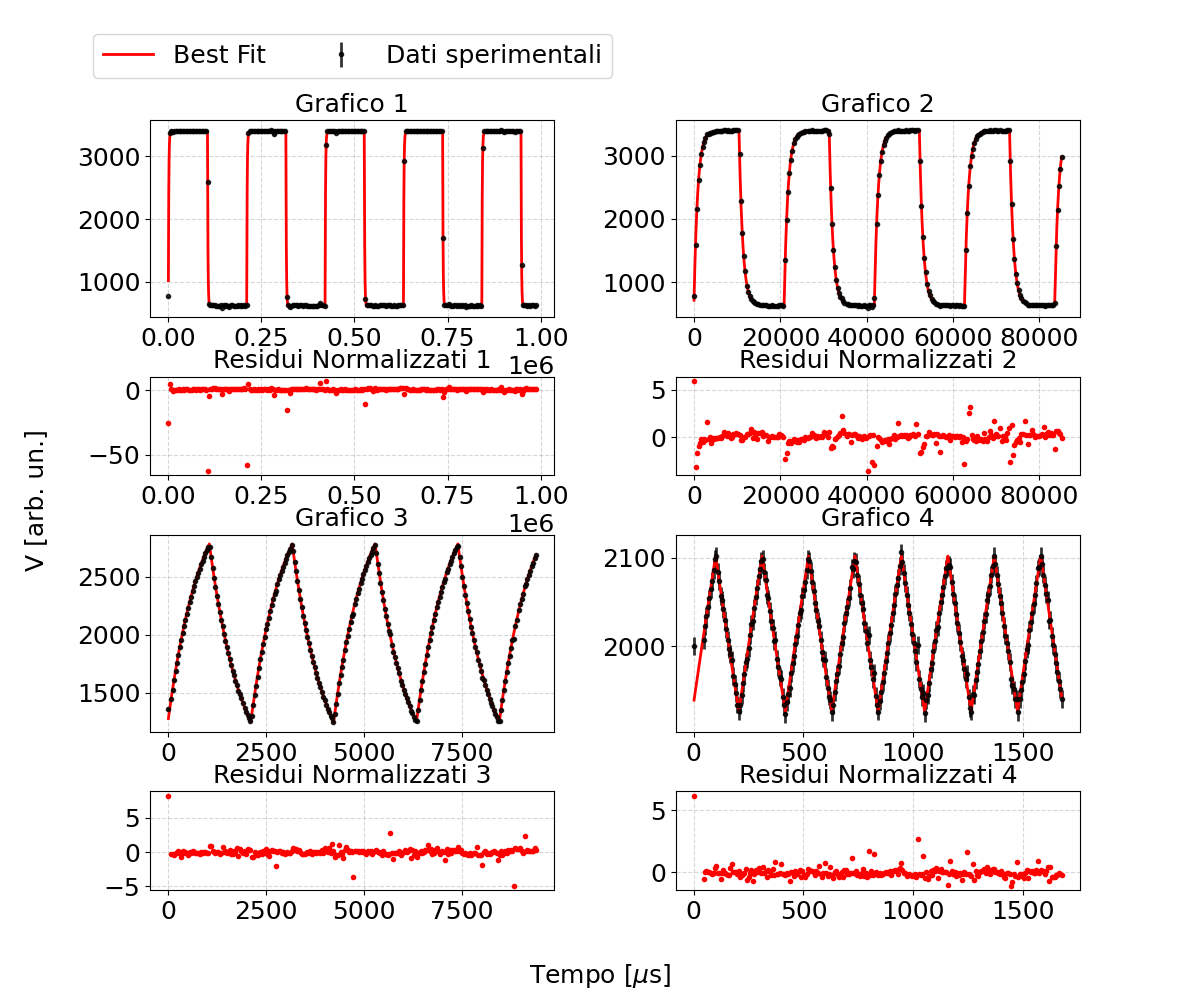
\includegraphics[width=1\textwidth]{bestfit_sharkfins.png} % Replace with your image name
                    \caption{.
                    }
                    \label{fig:bestfit_shark.fig}
                \end{figure}     

                \begin{table}[H]
                    \centering
                    \begin{tabular}{cccccc}
                        \hline
                         & Grafico1 & Grafico2 & Grafico3 & Grafico4 \\
                        \hline
                        $\omega$ [rad/s]    & $0.29839 \pm 0.0005$      & $300.691\pm 0.009$    & $2970.0 \pm 0.4$      & $29669.8\pm 0.2$ \\
                        $f_T$ [mHz]         & $0.140 \pm 0.001$         & $0.1864 \pm 0.0004$   & $0.189 \pm 0.002$     & $0.1 \pm 0.1$ \\
                        $\delta$ [$\mu$s]   & $178 \pm 3$               & $26 \pm 2$            & $10\pm 1$             & $6 \pm 1$ \\
                        a [arb.un]          & $2779\pm 1$               & $2767 \pm 2$          & $2746\pm 20$          & $4137\pm 4644$ \\
                        c [arb.un]          & $2090.0 \pm 0.6 $         &$2015.1\pm 0.6$        & $2025.9 \pm 0.6$      & $2014.8 \pm 0.6$ \\
                        $\chi^{2}_{norm}$   & 0.3                       &0.0071                 & 0.006                 & 0.007\\
                        \hline
                    \end{tabular}
                    \caption{Parametri ottenuti nei best-fit.}
                    \label{tab:bestfit_params}
                \end{table}
  

    \subsection{Onda sinusoidale}
        E' stato realizzato il best-fit dei minimi quadrati
        di quattro set di dati compatibile con un'onda sinusoidale.
        Il modello con cui fare il best-fit è descritto dall'Eq.($\ref{eq:fit_sin}$).
            \begin{equation}
                x(t)=a \sin\left(\omega t+\phi\right)
                \label{eq:fit_sin}
            \end{equation} 
        Dal $\chi^2$ risulta che l'errore è stato sovrastimato. 
        I parametri ottenuti sono riportati in Tab.(\ref{tab:bestfit_sinusoid}).%%%%%%%%%%%%%CHANGE TABLE 
        In Fig.($\ref{fig:bestfit_sinusoid}$) sono riportati i dati con il best fit e 
        i residui.

            \begin{figure}[H]            
                
                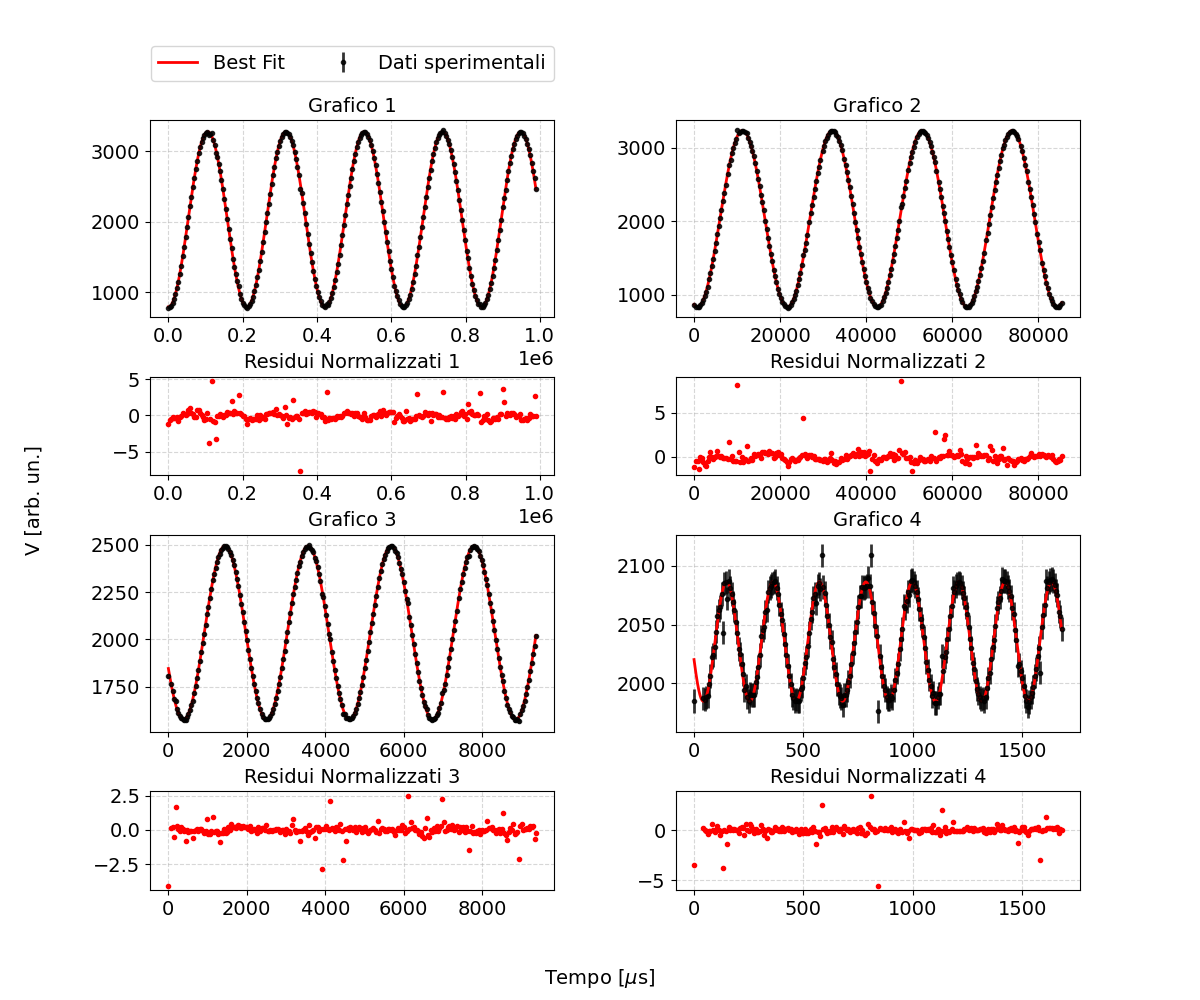
\includegraphics[width=1\textwidth]{bestfit_sinusoid.png} % Replace with your image name
                \caption{.
                }
                \label{fig:bestfit_sinusoid}
            \end{figure}    



            \begin{table}[H]
                \centering
                \begin{tabular}{cccccc}
                    \hline
                               & Grafico1              &Grafico2               & Grafico3                &Grafico4 \\
                    \hline
                    $\omega$ [rad/s]    & $29.822\pm 0.003$     & $300.77 \pm 0.03$     & $2969.9\pm 0.7$         & $29652  \pm 3$ \\
                    $\delta$ [$\mu$s]   & $-1.588 \pm 0.001$    & $-1.811 \pm 0.001$    & $-2.723\pm 0.004$       & $-2.89 \pm 0.04$ \\
                    a [arb.un]          & $1240.2\pm 0.8$       & $1201.2\pm 0.9$        & $459.0 \pm 0.8$         & $50.8 \pm 0.8$ \\
                    c [arb.un]          & $2035.9 \pm 0.6$      & $2036.5 \pm 0.6$      & $2035.3 \pm 0.6$        & $2035.4 \pm 0.6$ \\
                    $\chi^{2}_{norm}$   & 0.009                 & 0.009                 & 0.002                   & 0.004 \\
                    \hline
                \end{tabular}
                \caption{Parametri ottenuti nei best-fit.}
                \label{tab:bestfit_sinusoid}
            \end{table}

    \subsection{Onda triangolare}
        E' stato realizzato il best-fit dei minimi quadrati
        di quattro set di dati compatibile con un'onda traingolare.
         Il modello con cui fare il best-fit è descritto dall'Eq.($\ref{eq:fit_trian}$).
            \begin{equation}
                x(t) = a\sum_{k=1,3,5...}^{1000} G(f,f_T)\frac{4}{(k\pi)^2}\sin\left(k\omega (t+\delta)+\phi(f,f_T)\right) +c
                \label{eq:fit_trian}
            \end{equation} 
        Dal $\chi^2$ risulta che l'errore è stato sovrastimato. 
        I parametri ottenuti sono riportati in Tab.(\ref{tab:bestfit_triangle}).%%%%%%%%%%%%%CHANGE TABLE
        In Fig.($\ref{fig:bestfit_triangle}$) sono riportati i dati con il best fit e 
        i residui.

            \begin{figure}[H]            
                    
                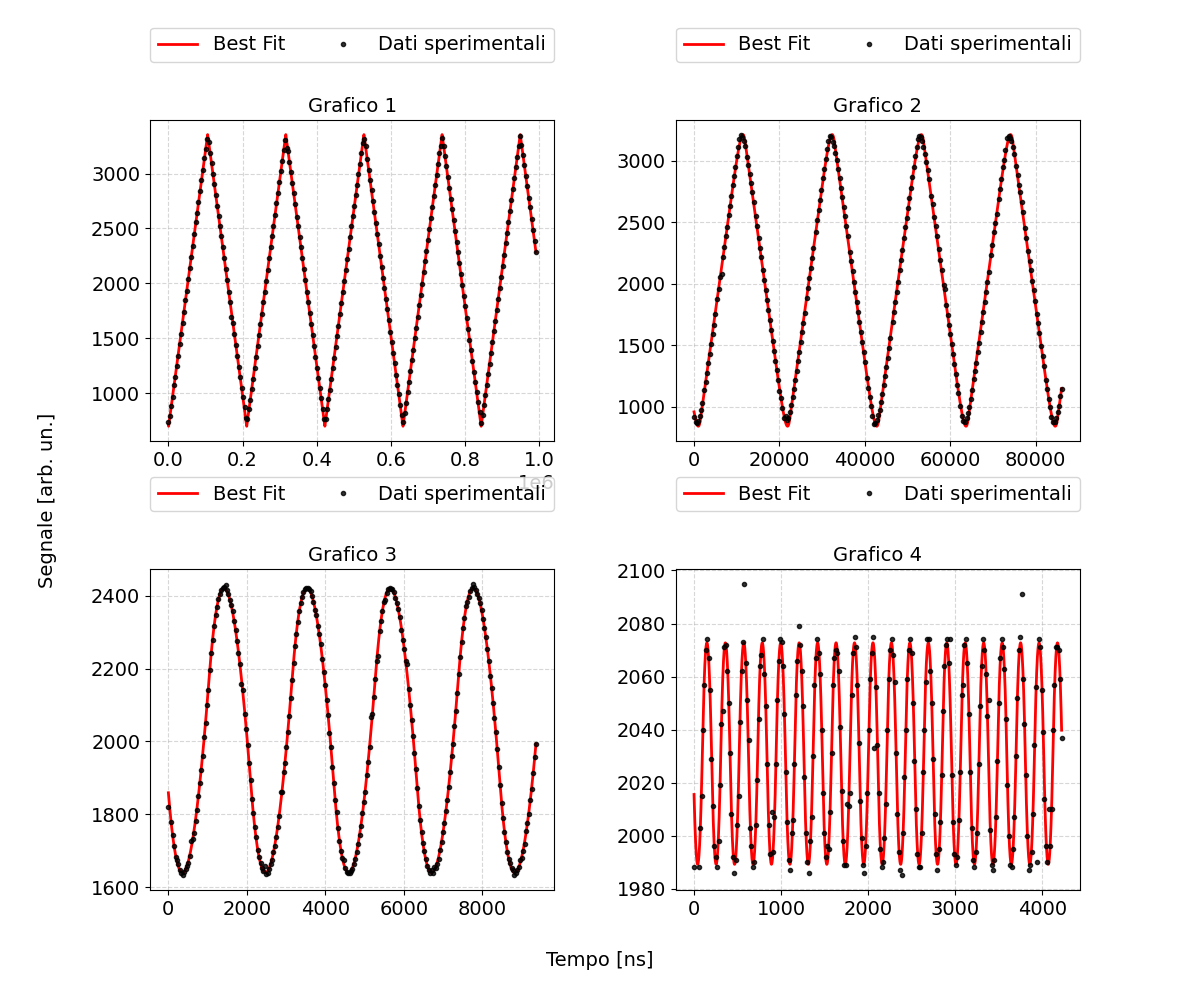
\includegraphics[width=1\textwidth]{bestfit_triangle.png} % Replace with your image name
                \caption{.
                }
                \label{fig:bestfit_triangle}
            \end{figure}    

            \begin{table}[H]
                \centering
                \begin{tabular}{cccccc}
                    \hline
                    Parametri           & Grafico1          &Grafico2               &Grafico3                   &Grafico4 \\
                    \hline
                    a [arb.un]          & $2665 \pm 3$      & $2671\pm 4$           & $2674\pm 139$             & $2652 \pm 12653$ \\
                    $\omega$ [rad/s]    & $29.817\pm 0.002$ & $300.784\pm 0.03$     & $2969.2\pm 0.08$          & $29667\pm 16$ \\
                    $\delta$ [s]        & $0.107\pm 0.002$  & $0.0105\pm 0.0001$    & $0.001073\pm 0.000007$    & $113\pm 7$ \\
                    c [arb.un]          & $2059.8 \pm 0.6$  & $1994.9 \pm 0.6$      & $2002.56 \pm 0.63$        & $2030.9 \pm 0.6$ \\
                    $f_T$ [$\mu$Hz]     & $61 \pm 4$        & $167 \pm 2$           & $187\pm 10$               & $189\pm 9$ \\
                    $\chi^{2}_{norm}$   & 0.007             & 0.006                 & 0.003                 & 0.0053 \\
                    \hline
                \end{tabular}
                \caption{Parametri ottenuti nei best-fit.}
                \label{tab:bestfit_triangle}
            \end{table}

    \subsection{Treno di impulsi}
        E' stato realizzato il best-fit dei minimi quadrati
        di un set di dati compatibile con un treno di impulsi.
            \begin{figure}[H]            
                        
                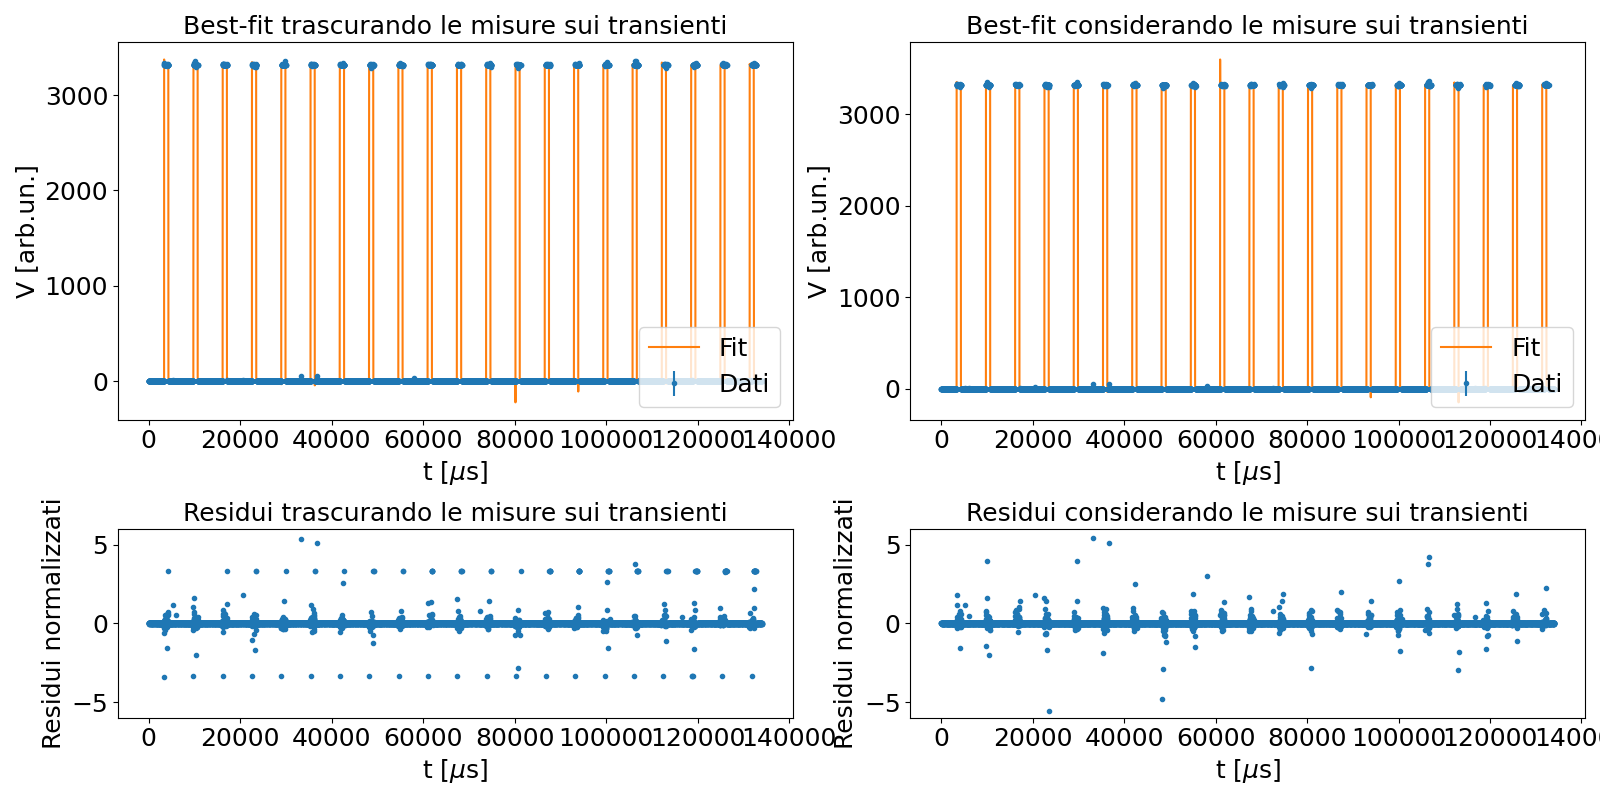
\includegraphics[width=1\textwidth]{bestfit_train.png} % Replace with your image name
                \caption{.
                }
                \label{fig:bestfit_train}
            \end{figure}    

            \begin{table}[H]
                \centering
                \begin{tabular}{ccc}
                    \hline
                               & Trascurando i transienti              &Considerando i transienti\\
                    \hline
                    a [arb.un]          & $3315 \pm 3$                          & $3312\pm 4$    \\
                    $\omega$ [rad/s]    & $981.7452\pm 0.0009$                  & $981.74\pm 0.04$ \\
                    $\delta$            & $0.145014\pm 0.000009$                & $0.14503\pm 0.00004$   \\
                    $\sigma$ [s]        & $-3870.016 \pm 0.002$                 & $-3869.9 \pm 0.3$  \\
                    $\chi^{2}_{norm}$   & 49                                    & 65 \\
                    \hline
                \end{tabular}
                \caption{Parametri ottenuti nei best-fit.}
                \label{tab:bestfit_triangle}
            \end{table}
\section{Simulazione numerica dei grafici guadagno vs frequenza}
        \begin{figure}[htbp]
            \centering
            \begin{subfigure}{0.45\textwidth} % Adjust width as needed
                \centering
                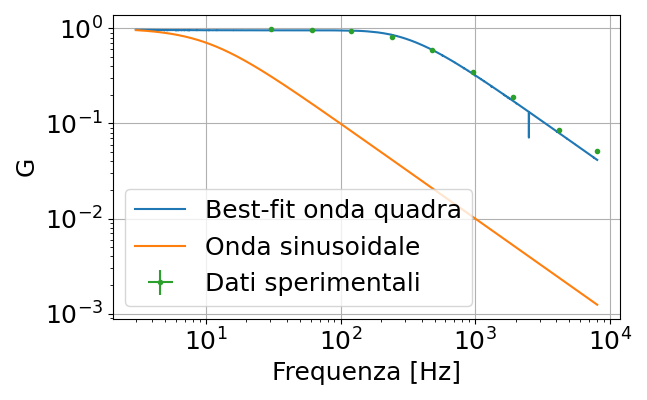
\includegraphics[width=\textwidth]{gain_squarewave.png} % Replace with your image path
                \caption{}
                \label{fig:image1}
            \end{subfigure}
            \hfill % Adds spacing between images
            \begin{subfigure}{0.45\textwidth} % Adjust width as needed
                \centering
                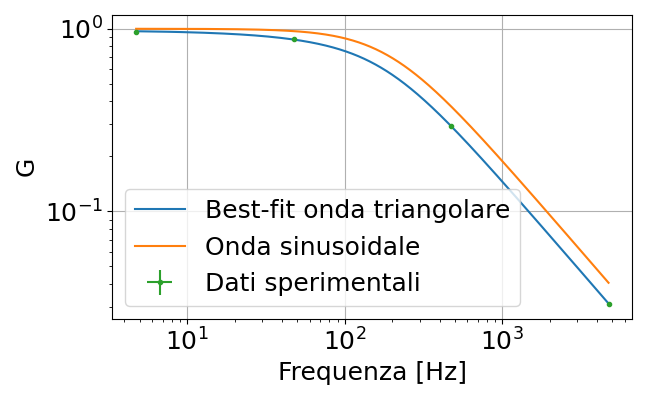
\includegraphics[width=\textwidth]{gain_trianwave.png} % Replace with your image path
                \caption{}
                \label{fig:image2}
            \end{subfigure}
            \caption{(a),(b)}
            \label{fig:side_by_side_images}
        \end{figure}


        \begin{table}[H]
            \centering
            \begin{tabular}{ccc}
                \hline
                            &Onda quadra        & Onda triangolare\\
                \hline
                $f_T$[$\mu$Hz]  &$191.6\pm0.9$      & $222\pm1$\\
                $a$         &$0.979\pm0.002$    &   $0.951\pm0.002$\\
                $K2$        & $52   $             &   $1$ \\
            
                \hline
            \end{tabular}
            \caption{}
            \label{tab:results}
        \end{table}
        \bibliographystyle{plain}
        \bibliography{main.bib}
\end{document}